\chapter{Literature Review}
\label{chapter:literatureReview}
\lhead{Chapter 2. \emph{Literature Review}}

Objectives for the MARISA project are well defined. In order to achieve the proposed goals and in preparation for this thesis a vast number of subjects were investigated. An investigation in the following theoretical topics : Behaviour analysis, Anomaly detection, Maritime safety technologies, were the major keywords for this literature review. 

In section \ref{section: Similar Frameworks} an analysis of the principal similar Frameworks found in the Literature, will be presented.
 A brief introduction to the maritime domain, regarding the Maritime Safety affairs is presented in section \ref{section: Maritime Safety}. In subsection ~\ref{subsection: chp2_AIS}, a description of the AIS technology and its use in the Maritime domain is presented.

\section{Maritime Safety}
\label{section: Maritime Safety}

Shipping is most likely, the most international task of all Worlds Industries, because of this international nature. It has long been recognized that improving maritime safety, is more effective if it is  carried out on a international level, than by individual countries acting unilaterally without any co-ordination, ~\cite{IMO2016}.

The UN (United Nations) in 1948, established the International Maritime Organization (IMO), as the first and principal international organization devoted to maritime matters. 

Since it's creation, the IMO has promoted the adoption of 50 conventions and protocols. The IMO has adopted more than 1000 codes and recommendations regarding the maritime safety and security.

The IMO objectives are easily summarized into their slogan : safe, secure, and efficient shipping on clean oceans.

\subsection{Automatic identification system (AIS)}
\label{subsection: chp2_AIS}
While the maritime safety domain is a vast and complex field for this investigation, it is important to focus on the technologies that the maritime domain has presented.

Automatic Identification System (AIS) is used to identify and locate Vessels by electronically exchanging data over high frequency VHF radio bandwidth to, other nearby ships and Vessel Traffic Services (VTS) stations.

The main motivation for the adoption of the AIS was its autonomous ability to identify other Vessels assisting humans with the collision avoidance. It has the ability to detect other equipped Vessel in situations where the radar detection is limited such as around bends, behind hills, and in conditions of restricted visibility by fog, rain, etc, ~\cite{Harati-Mokhtari2007}. 

In 2000, the IMO adopted a new requirement for all ships, to carry an automatic identification system (AIS) that automatically provides the Vessel information to coastal authorities and other Vessels.

This regulation was initially imposed for all international ships with 300 gross tonnage or more and for ships with 500 gross tonnage and upwards navigating not international voyages. After 31 of March 2014 all EU fishing Vessels above 15m, are obliged by the European Commission to install an AIS, ~\cite{EC2018}

The ships information sent over the AIS is classified into three main categories, they are presented in table:
\begin{table}[H]
\centering
\caption{AIS Information Description}
\label{Table: AIS Categories}
\begin{tabular}{|l|l|}
\hline
\textbf{Category} & \textbf{Description} \\ \hline
 & MMSI - Maritime Mobile Service Identity \\ \cline{2-2} 
 & IMO number \\ \cline{2-2} 
\textbf{Static Information} & Call sign and name \\ \cline{2-2} 
 & Type of ship \\ \cline{2-2} 
 & Length and beam \\ \cline{2-2} 
 & GPS Antenna location \\ \hline
 & Draught of ship \\ \cline{2-2} 
\textbf{Sailing Related Information} & Cargo information \\ \cline{2-2} 
 & Destination \\ \cline{2-2} 
 & ETA - Estimated Time of Arrival \\ \hline
 & Position of the ship \\ \cline{2-2} 
 & UTC - Coordinated Universal Time \\ \cline{2-2} 
 & COG - Course Over Ground \\ \cline{2-2} 
\textbf{Dynamic Information} & SOG - Speed Over Ground \\ \cline{2-2} 
 & Heading \\ \cline{2-2}
 & Navigational Status \\ \cline{2-2}
 & Rate of turn \\ \hline
\end{tabular}
\end{table}

Each Vessel transmits specific information related to the Vessel itself, the MMSI represents a 9 digit unique ID number, that every Vessel is assign with.
Most of the information sent over AIS, is automatically generated by the ships sensors such as the GPS and the compass. Thus minimizing the possibility of manipulate this data, although there is still information that is manually inserted by the crew such as the Navigational Status and the Heading.

Ships fitted with AIS are obliged to maintain the AIS in operation at all times. The AIS autonomously broadcast information, every certain time interval, therefore ships ping their AIS information every time interval   There are international agreements, that protect the navigational information.


\section{Behaviour Analysis}
Behaviour Analysis, is a vastly researched topic that involves many research fields. A vast number of Frameworks with the main objective of Maritime Behaviour Analysis are proposed in the literature, some of these frameworks are presented in section ~\ref{section: Similar Frameworks}.

For this work Vessel behaviour is as considered as a baseline in which abnormal behaviour can be found. This baseline occurs as normal trajectories are various and constant, producing a normalcy model of Vessels dynamics in which Machine Learning Techniques can learn.

Anomalies don't necessarily mean that there is something abnormal with the ship Vessel behaviour. That is something hard to imply with only AIS data. Anomalies in the AIS data can represent numerous abnormal events. Some of them that can be illegal, that's why further investigation from maritime authorities is needed. 

\subsection{Similar Frameworks}
\label{section: Similar Frameworks}

There are a vast number of frameworks in which Vessel behavior will be analyze. This will be done with the purpose of anomaly detection which are fully defined as integrated systems. The authors in ~\cite{Lei2016} suggested the framework MT-MAD (Maritime Trajectory Modelling and Anomaly Detection), in which a given set of moving objects, the most frequent movement behaviour are explored, evaluating a level of suspicion hence detecting anomalous behaviour.

The authors in ~\cite{Pallotta2013}, introduced the framework TREAD (Traffic Route Extraction and Anomaly Detection). The framework is proposed in which an Unsupervised Route Extraction is used to create a statistical model of maritime traffic from AIS messages, in order to detect low-likelihood behaviours and predict Vessels future positions.

A framework for Vessel behaviour analysis focusing on Vessel interaction or rendezvous. The proposed framework, is divided into the following three logical connected phases: Engagement Detection, Scenario  Detection and Anomaly Detection. The use of the 3-phase framework serves as a filter to reduce the volume of data that is processed by the sub-sequential phase. Therefore prioritizing critical scenarios, that request human intervention ~\cite{Shahir2015}.

Although accessing the performance of the frameworks, is an ardours task. There is no defined benchmark set where tests can be performed, with labeled samples described as positives or negatives of what are considered anomalies at seas ~\cite{Laxhammar2008}. 

In~\cite{Mao2016}, a detailed solution for constructing an AIS database, with the potential value for being used as benchmark database for maritime trajectory learning, and efficiency testing of data mining algorithms.

A partition-and-detect trajectory in which trajectories are partitioned into a two-level of granularity achieving high efficiency and high quality trajectory partitions, therefore detecting outlier trajectories using density-based methods, ~\cite{Lee}.

There are numerous studies that show how, Vessels tend to alter their routes in order to achieve safe distances when passing near other Vessel. In ~\cite{2017Offshore} a detailed study on Merchant Vessels AIS data, presents how this type Vessels alter their route, when new surface offshore petroleum installations are constructed.

\section{Trajectories Analysis}
\label{section: Trajectory Analysis}
Trajectories analysis is a researched field for numerous years. It is researched in areas where moving objects, this objects can be Humans, vehicles, animals, or even natural events such as hurricanes or storms.
A survey of trajectory data analysis applications, is presented in ~\cite{Feng2016}.

As the volume of positional AIS data exponentially increasing, it is important to find methods in witch raw trajectories data can produce value. This methods that learn with trajectory data can greatly impact the Maritime domain.

Trajectory learning is the process of learning motion-patterns from trajectory data using unsupervised techniques, mainly clustering algorithms ~\cite{LeGuillarme2013}.
Morris and Trivedi ~\cite{Morris2008}, further categorize trajectory learning as a three-step procedure: 

\begin{enumerate}
\item Trajectory Pre-Processing.
\item Trajectory Clustering. 
\item Path Modelling.
\end{enumerate}

In the Maritime domain, as Vessels are free to navigate in open waters, this fact produces a specific level of uncertainty related to Vessel trajectories, there are no standards for Vessel trajectory representation.

A way to discretize a trajectory discovering frequent regions is presented in ~\cite{Lei2016}. Representing the trajectories in a spatial grid in which a cell represents a geographical area with a defined size.

Pallotta, proposed a method that enriches the raw Vessels tracks with a description of the ship movements. This is the raw trajectories are labelled with the Vessel movement type information as 'Stationary' or 'Sailing' ~\cite{Pallotta2013}.

The authors in ~\cite{Lee}, raw trajectories are partitioned into sub-trajectories, creating a new insight for data analysis, adding the possibility of focused region analysis.  

A framework for scene modelling using trajectory dynamics analysis, for the discovery of POIs(Point of Interest) and the learning of AP(Activity Path), ~\cite{Morris2008}. 
These last representation is quite important for the Maritime domain, as the discovery of new POIs, can indicate the common Vessel destinations (e.g. frequent fishing zones, ports, etc.).  

\section{Time Series}
\label{section: Time Series}
The concept of time series is related to trajectories, as a time series is a set of ordered observations on a a quantitative characteristic of a
phenomenon at spaced time period, ~\cite{Ivanovic2016b}. Formally, a uni-variate time series $xj$, is defined as a sequence of real numbers, where $n$ is the length of the series, represented as:

\[xj = \left \{ x(i) \in \mathbb{R}: i = 1,2,3,...,n \right \} \]

 There are numerous applications for time series analysis, one of the main applications, is the use past time series, in order to forecast future values. These applications are used in numerous areas such as economics, engineering and others.


\subsection{Multivariate Time Series}
The AIS data cannot be described as a uni-variate times series, as it is composed by various variables. Therefore AIS data needs to be analyzed as a Multivariate Time Series (MTS).
For each AIS message, the features can be extracted with the timestamps that the message was broadcast. A detailed description of the AIS features is found in section ~\ref{subsection: chp2_AIS}. 

A possible representation of a Multivariate Time Series, $X$ is:
\[ X = (x_{1}, x_{2}, x_{3}, \cdots,x_{m}) \]

Where each $xj$ is defined in section ~\ref{section: Time Series}.

\[ Xj = \left \{ Xj(i) \in \mathbb{R}: i = 1,2,3,...,n \right \} (j = 1,2,3) \]

The analysis and classification of MTS is a arduous task for traditional machine learning algorithms, mainly because these algorithms do not handle well dozens of variables, ~\cite{MTS1}. Representing MTS into multiple univariate time series, can create losses in the correlation of these variables, as variables are being processed them independently.

\subsection{Time Series Clustering}
Temporal data mining research, a big emphasis lies on the clustering, and posterior classification of time series data. Time Series Clustering is used to identify in data-sets, homogeneous groups where same group object similarity is maximized, and the minimized when not in same group.  

The authors in ~\cite{WarrenLiao2005}, summarize previous work that investigates the clustering of time series applications in various fields, and propose an extensive survey. 

The same authors, define a necessity to clustering, when working with unlabelled data. This data can come from various sources including : categorical, numerical, images, spatial, e.t.c.

The main source of data for this work is AIS data, which is a  unlabelled multivariate data source. Labelled AIS data-sets for anomaly detection are either really expensive, or just not available for the public domain.  


\begin{figure}[H]
	\centering
	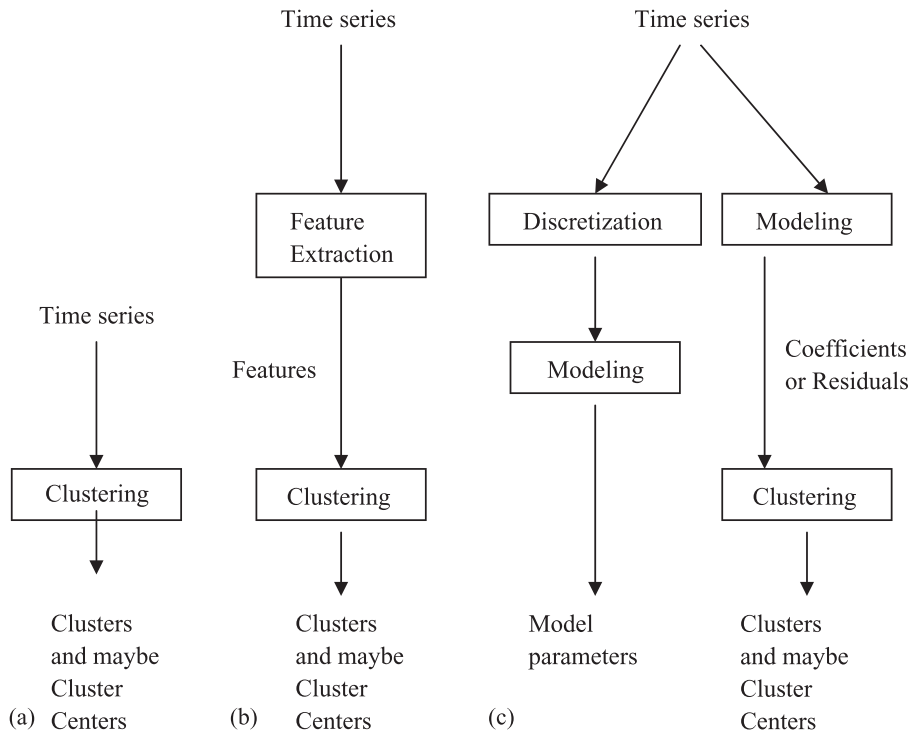
\includegraphics[scale = .6]{figures/TimeSeriesClustering}
    \caption{Three types of time series clustering defined in, ~\cite{WarrenLiao2005}}
    \label{fig:TimeSeriesClustering}
\end{figure}

Time Series Clustering can be categorized into three main general approaches, simply described in figure ~\ref{fig:TimeSeriesClustering}, these categories being:

\begin{itemize}
\item \textbf{Raw-data-based approaches (a)} These approaches work with raw sets of data, normally in the time domain. 

\item \textbf{Route Definition} Several methods of Vessel route definition, are presented in~\ref{chapter:literatureReview}.
Although, at this moment a method was chosen that represents the route as a whole. Therefore no information is lost, a detailed description of the latter is presented in~\ref{section: Trajectory Analysis}.

\item \textbf{Model-based approaches} This is a more complex clustering technique, in which, each Time-Series is considered as a statistical model or as a mixture of statistical distributions, thus two time series are considered similar when the models that fit this distributions are similar. 
\end{itemize}


%\todo{Needs completion for future work.}


\subsection{Time Series Classification}
Time series classification, is used for numerous purposes, from, the main difference when classifying or clustering Time Series lays in the fact that, classification can occur when a predefined set of classes already exist and the main objective is to classify this data in the different classes, thus in machine learning being considered a Supervised Learning task. 

Early work, from 1998, the authors propose p-value hypothesis test, performed for every pair of stationary multivariate time series, ~\cite{MTS1999}.

Three main categories of sequence time series classification, are defined by the authors in ~\cite{MTS_Classification}:

\begin{description}
\item[Feature Based Classification] A sequence of features is transformed into a feature vector, then convectional classification methods are applied. Feature selection represents is an important task for this method of classification.

\item [Distance Based Classification] The distance function that measures the
similarity between the time series, induce the quality of the classification overall. A more detailed research on these distances is presented in \cite{Knorr2000}.

\item [Model Based Classification] Where models, such as multivariate Gaussian mixture model (GMM) ~\cite{Laxhammar2008}, Support Vector Machines (SVM) or Hidden Markov Models (HMM) and other statistical models are used to classify time series.

\end{description}
 

\section{Distances Measures}
In order to compare classify a time series using distances, the concept of distance, and type of distance must be defined.

A distance is defined as a numerical measurement, that measures how far two objects are from each other. There are a vast number of distances used in computer algorithms. The most commonly used distance measure is the Euclidean distance, this measurement is a metric distance function, since it obeys to the three fundamentals metric properties: non-negativity, symmetry and triangle inequality ~\cite{Cai2004}. 

The similarity between two time series, can be calculated by simply summing the ordered point-to-point squared distance between both time series, this is shown in figure ~\ref{fig:EuclidianDTW}. 

Although, euclidean distance between two time series can only be calculated if, both time series are of equal length, ~\cite{EuclidianRef}. 
If two time series are identical, but one is shifted slightly along the time axis, using the Euclidean distance, it may consider the time series very different from each other, ~\cite{Salvador2007}.

This creates a problem when analyzing certain type of time series, as both may not have them same length, or might just be time-shifted, which happens when analyzing AIS data. In the literature a few solutions are presented, one of them is using another distance measure. 

\begin{figure}[H]
	\centering
	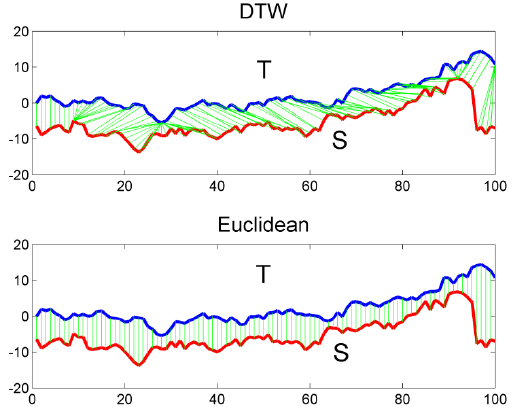
\includegraphics[scale = .5]{figures/DTWEuclidean.png}
    \caption{Difference between DTW distance and Euclidean distance (green lines represent mapping between points of time series T and S),~\cite{EuclidianRef}}
    \label{fig:EuclidianDTW}
\end{figure}


\subsection{Dynamic Time Warping (DTW)}
Dynamic Time Warping (DTW) is a algorithm that computes the optimal alignment and distance between two time series, ~\cite{Seto2015}. One time series may be “warped” non-linearly by stretching or shrinking it along its time axis.
%[GET A BETTER REF FOR THIS, NOT SALVADOR].

Although computing the DTW between two time series, is quite computationally expensive, has it's time and space complexity is $O(N^2)$, that limits its usefulness to only small time series with no more than 1000 points, ~\cite{Salvador2007}. 

As distance measures play an important role for similarity problem, in data mining tasks.








%\section{Data Fusion}
%\todo[inline]{Needs completion for future work. Depending on future work this might be needed.} 



